%%%%%%%%%%%%%%%%%%%%%%%%%%%%%%%%%%%%%%%%%%%%%%%%%%%%%%%%
%%%
%%%  LaTeX template for Junior Journal article
%%%  Please don't change next few lines
%%%
%%%%%%%%%%%%%%%%%%%%%%%%%%%%%%%%%%%%%%%%%%%%%%%%%%%%%%%%

\documentclass{juniorjournal}
%\setcounter{page}{}
%\journaltitle{}
%\volume{}
%\pubyear{}
%\licensee{}
%\authorlist{}
%\doi{}
%\articlenumber{}
%\articletype{}

%%%%%%%%%%%%%%%%%%%%%%%%%%%%%%%%%%%%%%%%%%%%%%%%%%%%%%%%
%%% 
%%%  List custom packages below, if needed. 
%%%  Note that amsfonts,amstext,amssymb,amsmath,amsthm,amscd
%%%  bm,paralist,color,graphicx,array and subfigure packages
%%%  are all part of juniorjournal.cls
%%%
%%%%%%%%%%%%%%%%%%%%%%%%%%%%%%%%%%%%%%%%%%%%%%%%%%%%%%%%

\usepackage{listings}
\usepackage{hyperref}

\definecolor{javared}{rgb}{0.6,0,0} % for strings
\definecolor{javagreen}{rgb}{0.25,0.5,0.35} % comments
\definecolor{javapurple}{rgb}{0.5,0,0.35} % keywords
\definecolor{javadocblue}{rgb}{0.25,0.35,0.75} % javadoc

\lstset{language=Java,
basicstyle=\ttfamily,
keywordstyle=\color{javapurple}\bfseries,
stringstyle=\color{javared},
commentstyle=\color{javagreen},
morecomment=[s][\color{javadocblue}]{/**}{*/},
numbers=left,
numberstyle=\tiny\color{black},
stepnumber=1,
numbersep=10pt,
tabsize=2,
frame=single,
breaklines=true
showspaces=false,
showstringspaces=false}

%%%%%%%%%%%%%%%%%%%%%%%%%%%%%%%%%%%%%%%%%%%%%%%%%%%%%%%%
%%%
%%%  Journal article basic info.
%%%  List all authors first and then their affiliations. 
%%%  Link author and affiliations with numbers in optional arguments.
%%%  For corresponding author use the form given below.
%%%  
%%%  For example:
%%%  \author[1]{Name1 Surname1}
%%%  \author[2, \corresp]{Name2 Surname2}\correspemail{email@edu.com}
%%%  \affil[1]{Institute1, Country1}
%%%  \affil[2]{Institute2, Country2}
%%%  
%%%%%%%%%%%%%%%%%%%%%%%%%%%%%%%%%%%%%%%%%%%%%%%%%%%%%%%%

\articletitle{LinkJVM 2.0 - Java on the KIPR Link} % To break lines in long titles use \\

%\author[ ,\corresp]{}\correspemail{}
\author[1, \corresp]{Markus Klein}\correspemail{m@mklein.co.at}
\author[1]{Christoph Hackenberger}
\affil[1]{Vienna Institute of Technology (TGM)}
%%%%%%%%%%%%%%%%%%%%%%%%%%%%%%%%%%%%%%%%%%%%%%%%%%%%%%%%
%%%
%%%  Main document.
%%%
%%%  To span floating objects (wide images, tables, etc.)
%%%  over twocolumn layout, use figure* 
%%%  or table* environments.
%%%
%%%  Examples:
%%%  \begin{figure*}	 \begin{table*}		
%%%   ...				  ...				
%%%  \end{figure*}		 \end{table*}		
%%%
%%%%%%%%%%%%%%%%%%%%%%%%%%%%%%%%%%%%%%%%%%%%%%%%%%%%%%%%

\begin{document}
\maketitle

\articleabstract{
One major part of any robot is his software.
The software brings the robot to life.
So it is really important that the software is powerful but at the same time it should be maintainable as easy as 
possible, especially when the program is written by a team.

Java is an object oriented programming language, which is not that hard to 
learn.
Unfortunately the KIPR Link does not support Java out of the box.

LinkJVM provides an open source full Java Runtime Environment(JRE) as well as an object oriented and easy to use library for controlling the robot.

The following paper shows a high and low level based implementation of a Java library for controlling the robot.
This is archieved by wrapping the native libkovan.
LinkJVM is also integrated into the KIPR Link's build system which allows easy and user-friendly deployment.
Further this papers describes of how to write programs in Java with the LinkJVM and how to get them 
running on the KIPR Link.
}

\keywords{Java, JVM, Botball, Library, Framework, Wrapper, KIPR Link, Libkovan, Robotic, JNI, SWIG, JamVM, GNU Classpath, Open Source}

\begin{figure*}[h]
\centering
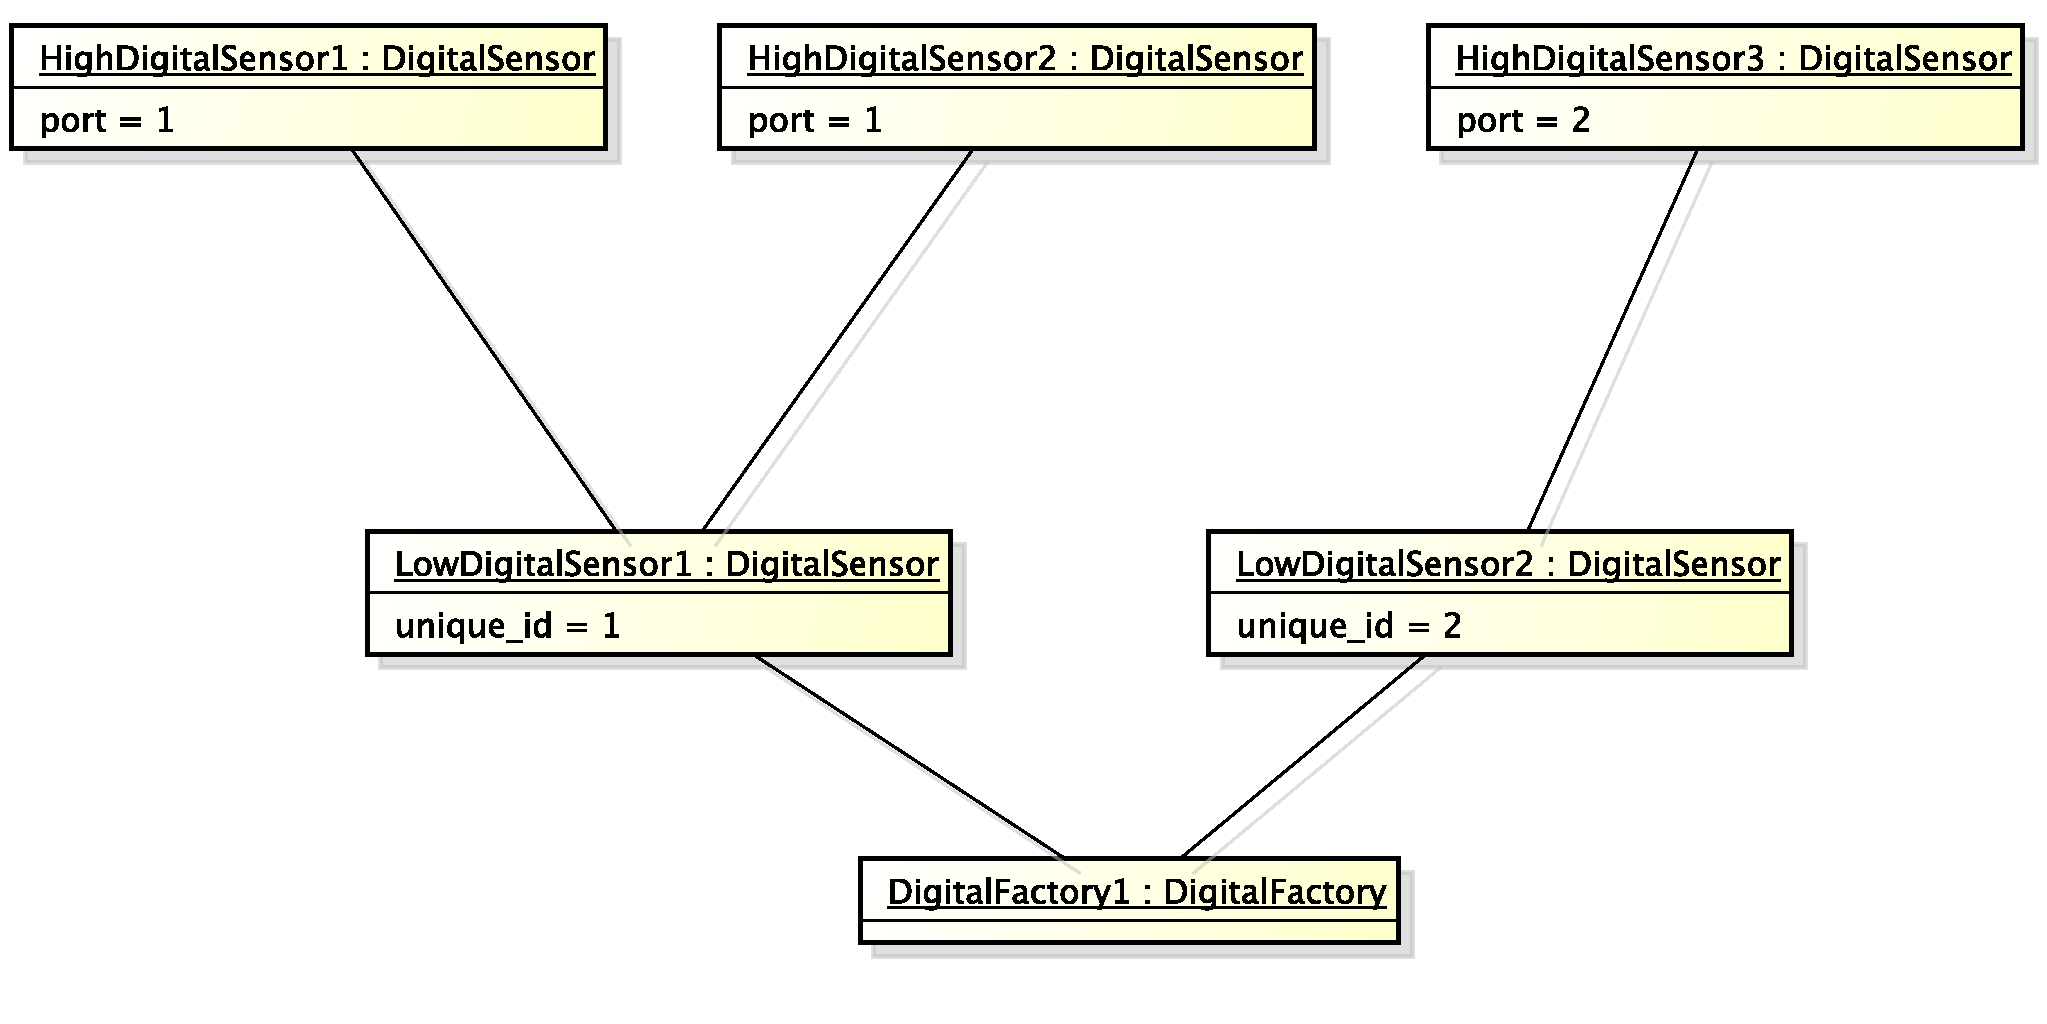
\includegraphics[width=0.8\textwidth]{images/Object-Diagram.pdf}
\caption{Object-Diagram showing a typical structure of a LinkJVM application}
\label{fig:Object-Diagram}
\end{figure*}

\section{Introduction}
The purpose of Botball\cite{Botball} is to motivate students for building and programming autonomous robots.
Most new students to Botball\cite{Botball} do not have any experience with programming.
Therefore the way of developing the robot software has to be very beginner friendly and easy to use, but especially in Austia where most botball students come from technical schools there is also a need for high level languages.

So what is the best language for Botball\cite{Botball}?
The authors do not think there is a best choice.
Every language has its own advantages and disadvantages.
C for example is a very powerful fast and processor-near language so it is quite good for a robot controller doing a lot of basic things such as controlling servos and motors, reading sensor values and so on. 
This is good for students without programming experience which only implement simple algorithms, but for more experienced students with more complex code C is not the right. 
While libkovan mostly avoids the real challenges or coding C, when implementing complex algorithms there is no way around pointers and memory management.

Another well-known possibility is Java\cite{Java}. 
Java\cite{Java} is much easier to learn and also pretty powerful and reliable.
Of course it is not as fast as compiled languages such as C or C++, but in the most cases it will make no real difference.
Java\cite{Java} is a higher level language than C which makes it in general easier to implement complex algorithms.
It provides automatic garbage collection to handle memory management 
and offers an excellent set of basic data structures such as lists, queues and maps as well as a huge standard library including easy to use APIs for network programming, multithreading and much more.
In C everything has to be built from scratch.
The object-oriented paradigm is also very helpful to structure the program 
to improve the maintainability, especially in bigger projects.
Moreover Java is compiled into cross platform bytecode instead of target specific machine code, so Java programs do not need to be compile directly on KIPR Link.

In most schools in Austria students get started with programming using Java\cite{Java} and not C or C++.
Therefore the authors would consider themselves as a good Java\cite{Java} programmer, 
but they never wrote a bigger project using C nor C++.

Further alternatives are event-based frameworks using a scripting language 
such as node\cite{node} or in general scripting languages, but these can be implemented very easily, 
because the JVM\cite{JVM}(Java\cite{Java} Virtual Machine) supports a huge amount of additional languages 
including javascript, scala and clojure.

\section{State of the Art}
LinkJVM 1.0\cite{linkjvm1.0} was published at the Global Conference on Educational Robotics 2013 (GCER\cite{GCER} 2013).
While the Java\cite{Java} environment JamVM and GNU Classpath\cite{GNU} work pretty well the robot library is not that good.
At that time LinkJVM 1.0\cite{linkjvm1.0} wraps over libkovan's\cite{libkovan} C bindings which makes the libary structure pretty poor, because LinkJVM 1.0\cite{linkjvm1.0} first calls the native C function and then the native C function manages the C++ objects.
This approach is easier to implement, but it also comes with some downsides.
The most important of them is that there no possibility to write a thread save library using this approach, because libkovan\cite{libkovan} itself is not thread-save.
Moreover LinkJVM 1.0\cite{linkjvm1.0} offers only a very small API with much less features that libkovan\cite{libkovan} does and LinkJVM's 1.0\cite{linkjvm1.0} vision system contains also just one camera class.
Therefor the authors decided to write a new library from scratch, which will fix all this issues. 

\section{Design Approach}
\label{sec:design-approach}
The framework of the LinkJVM consists of one high and one low level part.
The low level part of the LinkJVM wraps the existing C++ library of libkovan\cite{libkovan}, 
the high level now wraps the low level part and represents the API for the user.
So the user only uses the high level part of the LinkJVM and should not come in 
contact with any low level things.

\begin{figure}[H]
\centering
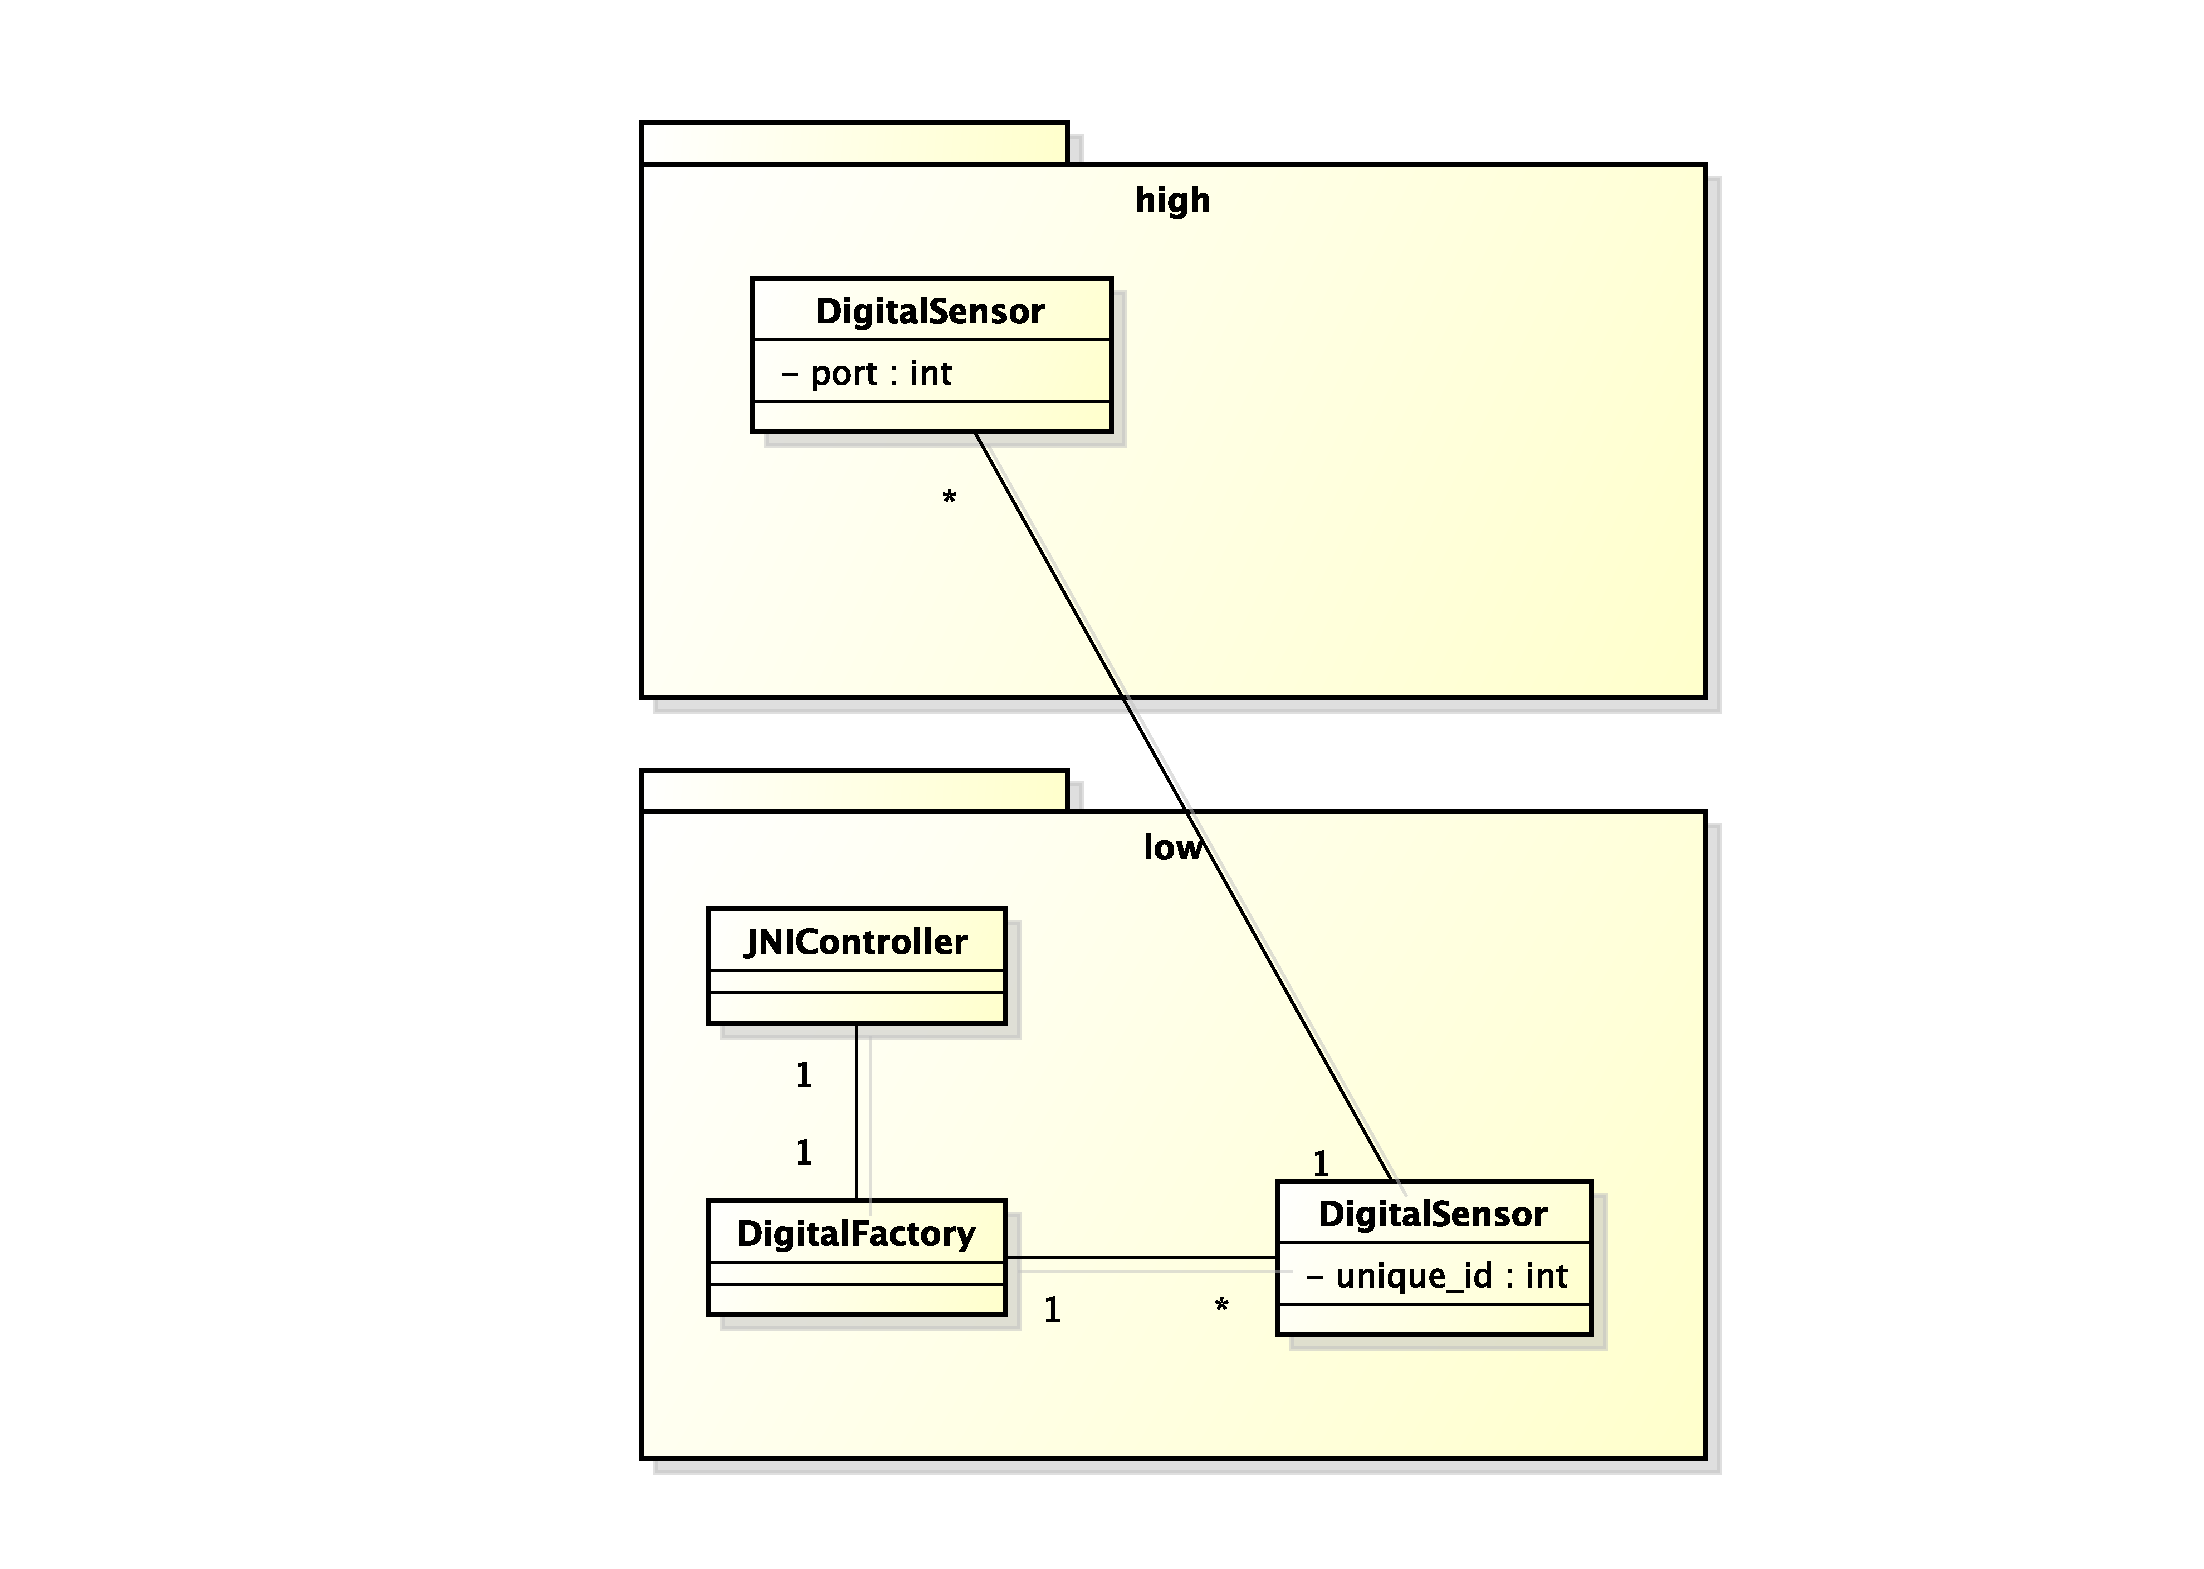
\includegraphics[width=0.4\textwidth]{images/Class-Diagram.pdf}
\caption{Class-Diagram showing the releationships or the different high and low level components}
\label{fig:Class-Diagram}
\end{figure}

For example the user has a digital sensor like a lever on his robot and now 
wants to use this sensor in his program. He will now create a new high level 
DigitalSensor object, which uses a low level DigitalSensor object in the 
background (see Figure \ref{fig:Class-Diagram}) that again uses the C++ implementation of a DigitalSensor.

The user can create as much high level objects of the same sensor, motor, 
servo,... , which will all uses the same low level object with the specified 
unique identifier, which is for example the port of a sensor. If the user 
creates a new high level object with a unique identifier that is unequal to 
an existing low level object the appropriate factory would 
create a new low level object with the specified unique identifier. (see figure \ref{fig:Object-Diagram})

Both the low and the high level parts are described in detail in the following subsections:

\subsection{Low Level}
The low level part of the framework contains the Java\cite{Java} side libkovan\cite{libkovan} wrapper. 
Every object of a low level class is also a native C++ object.
This classes must be instantiated using the corresponding multiton factory, which means that every low object has a unique identifier as described in section \nameref{sec:design-approach}.
The low level part also provides the JNIController class which holds a singleton of every factory as well as one static singleton object of itself.
Most low level parts are automatically generated wrapper classes using the Simplified Wrapper and Interface Generator(SWIG\cite{SWIG}).
This software generates the Java\cite{Java} and the C++ wrapper out of an interface file with all class definition that should be wrapped.

\subsection{High Level}
The high level part contains, as already mentioned before, the object oriented API for the user. 
Internally every time the user creates a new high level object, the high object requests a new low object.
See Figure \ref{fig:Class-Diagram} and Figure \ref{fig:Object-Diagram}.

\section{LinkJVM - API}
The API of LinkJVM (or the robot libary) provides a object oriented, well documented , easily to use and maintainable library for controlling the KIPR\cite{KIPR} Link\cite{link}
 and all its connected devices.
The API contains classes for the following components:
\begin{itemize}
	\item iRobot Create\cite{create}
	\item motors and servos
	\item analog and digital sensors
	\item hardware and software buttons
	\item vision system
	\item depth camera (experimental)
	\item AR.Drone 1.0/2.0\cite{ar.drone}
\end{itemize}
The most important components of the framework are described in detail in the following subsections.

\subsection{Botball Class}
The Botball\cite{Botball} Class contains some basically static methods like shutDownIn, 
waitForLight or msleep.
The next listing shows the usage of these methods:
\lstinputlisting[caption={Usage of the Botball class}, language=Java]{listings/botball_class.java}

\subsection{Motors/Servos and Sensors}
LinkJVM's robot libary provides classes for the different types or motors, servos and sensors.
The following listing shows the usage of motors and sensors:
\lstinputlisting[caption={Basic usage of sensors and motors}, language=Java]{listings/drive_until_bump.java}
The example above shows a very simple program, which let the robot drive forward 
until a digital sensor which is used as bump sensor bumps.

\subsection{Create}
The iRobot Create\cite{create} is a very good example to show the advantage of the usage of 
an object oriented programming language like Java\cite{Java}.
The following example shows the usage of the iRobot Create\cite{create}:
\lstinputlisting[caption={Usage of the iRobot Create with LinkJVM}, language=Java]{listings/create_roomtour.java}
With this code it is possible to do a room tour with the iRobot Create\cite{create}.
After the start button was pressed the Create\cite{create} starts moving until it bumps, then 
it turns and moves on in another direction. The program runs until the side 
button on the KIPR\cite{KIPR} Link\cite{link} is pressed.

\subsection{Vision System}
The LinkJVM's vision system consists basically of 3 major classes(see figure \ref{fig:Vision-System}):
\begin{itemize}
	\item {\bf ImageProcessor}: The ImageProcessor processes the image to color or QR blobs with a given CameraConfig and a given channel number and proviedes afterward the CameraObjects. 
	\item {\bf CameraObject}: One CameraObject represents an object tracked by an image processor. It contains information like the bounding box or the center point about the blob.
	\item {\bf CameraConfig}: An CameraConfig object contains several configuration attribute for an ImageProcessor.
\end{itemize}
\begin{figure}[H]
\centering
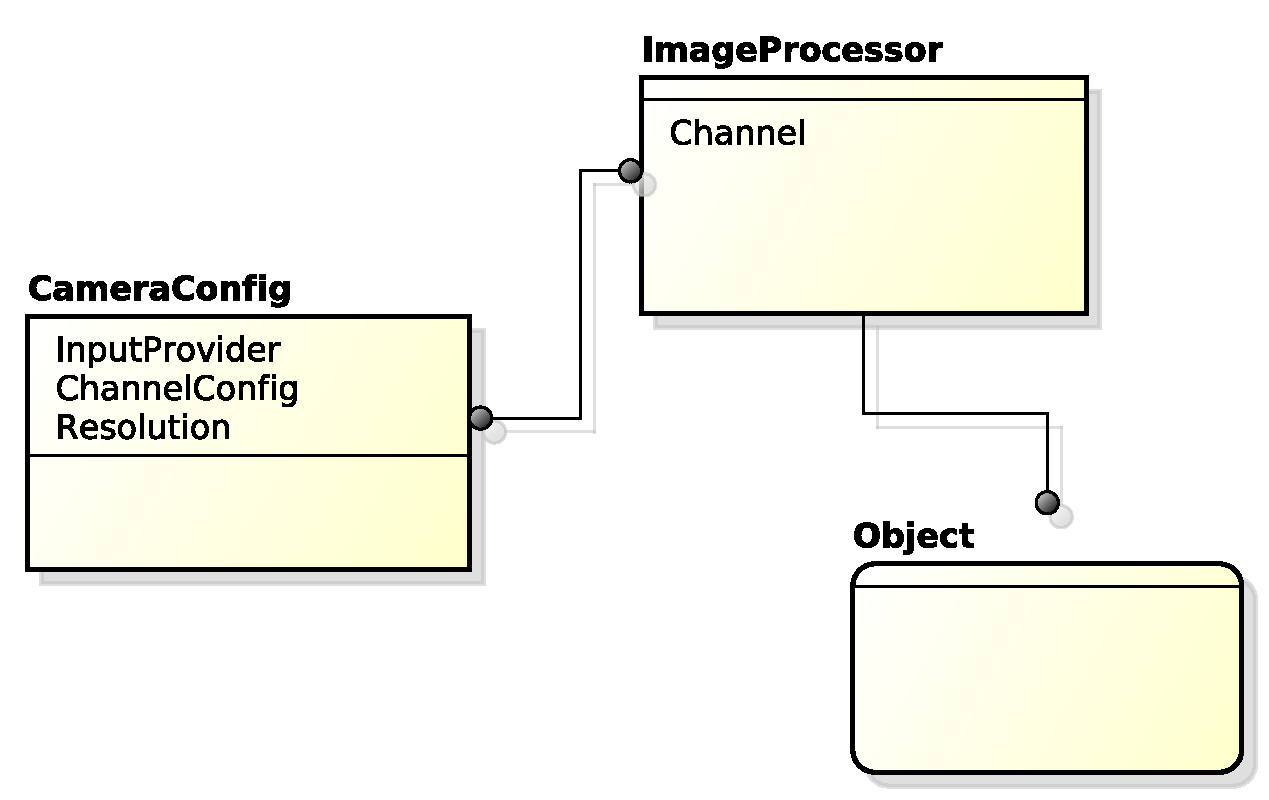
\includegraphics[width=0.5\textwidth]{images/vision.pdf}
\caption{Overview over LinkJVM's Vision System}
\label{fig:Vision-System}
\end{figure}
\lstinputlisting[language=Java, caption={Basic usage of the vision system}]{listings/vision.java}

\subsection{Debugger}
The LinkJVM-Debugger allows the user to send debug message over the network to a debugger client.
Therefore the API provides a debugger class which connects establishes a connection to a client.
\lstinputlisting[language=Java, caption={Example usage of the LinkJVM-Debugger}]{listings/Debugger.java}

\section{Java Environment}
LinkJVM includes a Java\cite{Java} Runtime Environment(JRE\cite{JRE}) which consists of a lightweight Java\cite{Java} Virtual Machine(JVM\cite{JVM}) and GNU Classpath\cite{GNU} an open source implementation of the Java\cite{Java} core classes.
So LinkJVM 2.0 uses basically the same Java\cite{Java} environment than LinkJVM 1.0\cite{linkjvm1.0} does, but in addition LinkJVM 2.0 offers the \frqq eclipse Java\cite{Java} compiler\flqq  as Java compiler (javac) and the \frqq jar\flqq  for packaging multiple class files.
Using these tools Java\cite{Java} programs can be directly compiled and packaged on the KIPR Link, but since class and jar files contain cross platform bytecode, it is not necessary to compile the programs on the KIPR Link. (See section \nameref{sec:developing-tools})

\section{Integration into KIPR Link's build system}
The KIPR\cite{KIPR} Link\cite{link} is based on a build framework called \frqq OpenEmbedded\flqq\cite{openembedded} and its accociated build system \frqq bitbake\flqq  which provides a cross compile environment for embedded Linux\cite{Look_Inside_Kipr_Link}.
Unfortunately the KIPR\cite{KIPR} Link\cite{link} does not work with the latest version of these tools, so building the firmware or adding packages is very hard.
Furthermore OpenEmbedded\cite{openembedded} only works on Linux machines and also requires knowledge of basic and moderately complex terminal commands.
Fortunately with the excellent help of KIPR staff, the authors managed to set up a build server and compile a LinkJVM package.

\subsection{LinkJVM's build system}
As already mentioned before LinkJVM's source consists of a C++ and a Java\cite{Java} part.
To combine both build processes using only one build system the authors decided to use CMake for compilation.
CMake is an open source, cross platform build system which supports C++ as well as Java\cite{Java} and automatically generates makefiles.

For integration into KIPR\cite{KIPR} Link's\cite{link} build system the authors added an meta-layer which provides a bitbake recipes for building LinkJVM.

\subsubsection{Deployment}
Using bitbake LinkJVM is compiled and packaged into a ipk software package which can be easily installed on the Link\cite{link} directly via BotUI.

It is also possible to directly add LinkJVM to a firmware image and in the future LinkJVM may also be integrated into the offical Link\cite{link} firmware.
\section{Developing Tools}
\label{sec:developing-tools}
Because the code the user writes with the LinkJVM library uses the programming 
language Java\cite{Java}, it is not possible to use the KISS IDE from KIPR\cite{KIPR} because it only 
supports C or C++ code.

The authors decided to leave the choice of how to write the code at the user. It 
is possible to write the code with an IDE like Eclipse or Netbeans or just write 
it in a simple text editor and compile the source code over the console.

\begin{figure}[H]
\centering
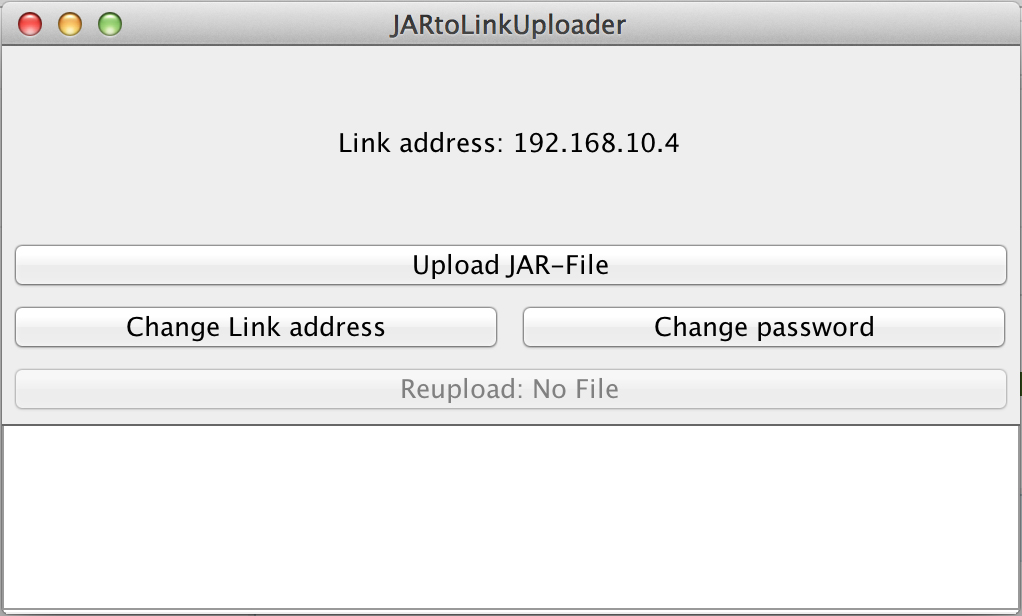
\includegraphics[width=0.5\textwidth]{images/linkjvm_uploader.jpg}
\caption{LinkJVM-Uploader}
\label{fig:linkjvm_uploader}
\end{figure}

At the beginning it was only possible to upload/run the users program via scp/ssh to/on the KIPR\cite{KIPR} Link\cite{link}.
Running a program over ssh is not tournament-conformal, so the only thing that could be done 
was to write a C wrapper, which executes your Java\cite{Java} program.

So the next logical thing the authors have to think about is how to get the compiled 
program on the KIPR\cite{KIPR} Link\cite{link} and make it run able there in a for the user easy way?
They first thought about a plugin for the Eclipse IDE but this would extremely 
limit the user of how to write the code, which like already mentioned the 
authors wanted to leave the choice at the user.
The authors decided to write an independent program, which is called 
LinkJVM-Uploader or JARtoLinkUploader (see Figure \ref{fig:linkjvm_uploader}), 
to upload .jar files to the Link\cite{link}. This program also automatically creates C 
wrappers, which executes the .jar files and which are shown in the menu point 
\frqq Programs\flqq  on the KIPR\cite{KIPR} Link\cite{link}. All this is done over ssh and scp connections in 
the background.

\section{Conclusion}
LinkJVM 2.0 comes with a completely new robot library which fixes many problems of LinkJVM 1.0\cite{linkjvm1.0}.
Now the user does not have care of the thread safety and the vision system provides an excellent API for using the KIPR\cite{KIPR} Link's\cite{link} camera. 
Since LinkJVM has also been integrated into the KIPR\cite{KIPR} Link's\cite{link} build it is incredibly easy to install and upgrade which makes it pretty attractive for Botball students.
Although the design approach shown in this paper works very good, it is still not perfect,
especially because developing on the core of LinkJVM requires advanced knowledge 
of the Java\cite{Java} Native Interface(JNI), which makes it pretty hard for students to fix bugs on their own.
Moreover since there are very few people with a build server compiling LinkJVM is nearly impossible.

So the next logical step would be to make LinkJVM's robot library a pure Java\cite{Java} library and replace the low level part with real implementation.
This could be archived pretty easy, because the most parts of libkovan\cite{libkovan} does nothing else than communicates with the kovan kmod via UDP. 
The kovan kmod is a kernel module which provides an interface to KIPR\cite{KIPR} Link's\cite{link} FPGA.
Using this approach, LinkJVM could also be built without an build server, because it would only consist cross platform bytecode. 

\begin{thebibliography}{500} % Include .bib (.bbl) references here
\bibitem{Java}
  Java, Oracle,
  http://www.java.com/en/, March 2014
\bibitem{KIPR}
  KISS Institute for Practical Robotics,
  http://www.kipr.org, 2014
\bibitem{Botball}
  Botball, Standards-Based Educational Robotics Program, 
  http://www.botball.org, 2014
\bibitem{node}
  Node Javascript, 
  http://nodejs.org/, March 2014
\bibitem{JVM}
  JVM, Java Virtual Machine,
  http://en.wikipedia.org/wiki/Java\_virtual\_machine, March 2014
\bibitem{JRE}
  JRE, Java Runtime Environment, 
  http://www.oracle.com/technetwork/java/javase/
  downloads/, March 2014
\bibitem{linkjvm1.0}
  Klein Markus: \frqq Java on the KIPR Link\flqq  ,
  http://files.kipr.org/gcer/2013/proceedings/
  Klein\_Java\_KIPR\_Link.pdf, 2013
\bibitem{libkovan}
  McDorman B.: libkovan C standard library,
  https://github.com/kipr/libkovan, March 2014
\bibitem{GCER}
  GCER, Global Conference on Educational Robotics,
  http://www.kipr.org/gcer, 2014
\bibitem{GNU}
  GNU Classpath, open source Java core class implementation,
  http://www.gnu.org/software/classpath/, March 2014
\bibitem{Look_Inside_Kipr_Link}
  Braden McDorman, Joshua Southerland: \frqq A Look Inside the KIPR Link\flqq  ,
  http://files.kipr.org/gcer/2013/proceedings/
  McDorman\_A\_Look\_Inside\_the\_KIPR\_Link.pdf, 2013
\bibitem{create}
  iRobot Create, Programable Robot,
  http://www.irobot.com/us/learn/Educators/Create.aspx, March 2014
\bibitem{ar.drone}
  AR.Drone, Parrot,
  http://ardrone2.parrot.com, March 2014
\bibitem{link}
  Link, Robot Controler,
  http://www.kipr.org/products/link, March 2014
\bibitem{openembedded}
  OpenEmbedded, build framework for embedded Linux,
  http://www.openembedded.org/wiki/Main\_Page, March 2014
\bibitem{SWIG}
  SWIG, Simplified Wrapper and Interface Generator,
  http://www.swig.org, March 2014
\end{thebibliography}

\end{document}
